\section{Auswertung}
\label{sec:Auswertung}

Aus den Messwerten wird zunächst die Molwärme für konstanten Druck $C_p$ errechnet. Anschließend wird diese in die Molwärme bei 
konstanten Volumen $C_V$ umgerechnet. Aus den beiden Molwärmen wird die Debye-Temperatur $\theta_\text{D}$ bestimmt. Um diesen 
vergleichen zu können, wird ein theoretischer Wert für $\theta_\text{D}$ berechnet. 

\subsection{Bestimmung von $C_p$ und $C_V$}

Um $C_p$ zu bestimmen wird 

\begin{equation*}
    C_p = \frac{U I \symup{\Delta}t M}{\symup{\Delta} T m}
\end{equation*}

verwendet. Dabei ist $U$ die Heizspannung, $I$ der Heizstrom, $\symup{\Delta}t$ das Heizintervall, $M = \SI{63.5}{\gram\per\mole}$ die molare Masse \cite{Molare}, 
$\symup{\Delta}T$ die Temperaturerhöhung und $m = \SI{342}{\gram}$ \cite{Anleitung} die Masse der Probe. Für Kupfer werden weiterhin die Dichte $\rho = \SI{8.96}{\gram\per\cubic\centi\meter}$
\cite{KompDichte} und der Kompressionsmodul $\kappa = \SI{137.8}{\giga\pascal}$ \cite{KompDichte} angenommen.\\

Für $C_p$ ergeben sich die Werte in Tabelle \ref{tab:mess1}. Mithilfe von Gleichung \eqref{eqn:Temp} sind die Temperaturen umgerechnet worden. 

\begin{table}
    \centering
    \caption{Messwerte zur Berechnung der Molwärme bei konstantem Druck $C_p$. Die Temperaturen wurden dabei aus \eqref{eqn:Temp} berechnet.}
    \label{tab:mess1}
    \sisetup{table-format=2.1}
    \begin{tabular}{c c c c c c}
    \toprule
    $T_\text{Probe} \,/\, \si{\kelvin}$ & $T_\text{Gehäuse} \,/\, \si{\kelvin}$ & $U \,/\, \si{\volt}$
    & $I \,/\, \si{\milli\ampere}$ & $\symup{\Delta}t \,/\, \si{\second}$
    & $C_p \,/\, \si{\joule\per\kelvin\mole}$\\
    \midrule 
         81,06 &  80,82 & 0,00 & 00,0 & 0 & \\
         81,76 &  88,13 & $\num{5.29+-0.5}$ & $\num{50.5+-0.5}$ & $\num{ 76+-2}$ & $\num{0.59+-0.06}$\\
         86,71 &  95,23 & $\num{5.34+-0.5}$ & $\num{50.9+-0.5}$ & $\num{284+-2}$ & $\num{1.68+-0.16}$\\
         91,92 & 102,12 & $\num{5.36+-0.5}$ & $\num{51.1+-0.5}$ & $\num{176+-2}$ & $\num{0.88+-0.08}$\\
         99,03 & 108,31 & $\num{5.39+-0.5}$ & $\num{51.3+-0.5}$ & $\num{281+-2}$ & $\num{1.55+-0.15}$\\
        106,17 & 116,19 & $\num{5.41+-0.5}$ & $\num{51.4+-0.5}$ & $\num{269+-2}$ & $\num{1.38+-0.13}$\\
        112,13 & 123,87 & $\num{5.42+-0.5}$ & $\num{51.5+-0.5}$ & $\num{220+-2}$ & $\num{0.97+-0.09}$\\
        119,55 & 131,34 & $\num{5.43+-0.5}$ & $\num{51.6+-0.5}$ & $\num{278+-2}$ & $\num{1.23+-0.11}$\\
        124,59 & 139,07 & $\num{5.44+-0.5}$ & $\num{51.6+-0.5}$ & $\num{169+-2}$ & $\num{0.61+-0.06}$\\
        133,51 & 147,31 & $\num{5.45+-0.5}$ & $\num{51.7+-0.5}$ & $\num{274+-2}$ & $\num{1.04+-0.10}$\\
        140,28 & 155,58 & $\num{5.46+-0.5}$ & $\num{51.7+-0.5}$ & $\num{230+-2}$ & $\num{0.79+-0.07}$\\
        148,28 & 163,89 & $\num{5.47+-0.5}$ & $\num{51.7+-0.5}$ & $\num{228+-2}$ & $\num{0.77+-0.07}$\\
        158,75 & 172,71 & $\num{5.47+-0.5}$ & $\num{51.8+-0.5}$ & $\num{320+-2}$ & $\num{1.21+-0.11}$\\
        167,07 & 180,59 & $\num{5.48+-0.5}$ & $\num{51.8+-0.5}$ & $\num{233+-2}$ & $\num{0.91+-0.08}$\\
        173,21 & 190,22 & $\num{5.50+-0.5}$ & $\num{51.8+-0.5}$ & $\num{223+-2}$ & $\num{0.69+-0.06}$\\
        179,11 & 200,40 & $\num{5.49+-0.5}$ & $\num{51.9+-0.5}$ & $\num{147+-2}$ & $\num{0.37+-0.03}$\\
        187,26 & 208,62 & $\num{5.49+-0.5}$ & $\num{51.9+-0.5}$ & $\num{184+-2}$ & $\num{0.46+-0.04}$\\
        197,17 & 217,37 & $\num{5.49+-0.5}$ & $\num{51.9+-0.5}$ & $\num{240+-2}$ & $\num{0.63+-0.06}$\\
        205,63 & 227,41 & $\num{5.50+-0.5}$ & $\num{51.9+-0.5}$ & $\num{211+-2}$ & $\num{0.51+-0.05}$\\
        213,87 & 238,51 & $\num{5.50+-0.5}$ & $\num{51.9+-0.5}$ & $\num{175+-2}$ & $\num{0.38+-0.03}$\\
        224,40 & 250,67 & $\num{5.50+-0.5}$ & $\num{51.9+-0.5}$ & $\num{186+-2}$ & $\num{0.38+-0.03}$\\
        233,46 & 258,81 & $\num{5.50+-0.5}$ & $\num{51.9+-0.5}$ & $\num{166+-2}$ & $\num{0.35+-0.03}$\\
        243,31 & 268,01 & $\num{5.50+-0.5}$ & $\num{51.9+-0.5}$ & $\num{173+-2}$ & $\num{0.37+-0.03}$\\
        251,18 & 275,95 & $\num{5.50+-0.5}$ & $\num{52.0+-0.5}$ & $\num{131+-2}$ & $\num{0.28+-0.03}$\\
        258,81 & 283,92 & $\num{5.49+-0.5}$ & $\num{52.0+-0.5}$ & $\num{120+-2}$ & $\num{0.25+-0.02}$\\
        272,10 & 292,95 & $\num{5.49+-0.5}$ & $\num{51.9+-0.5}$ & $\num{208+-2}$ & $\num{0.53+-0.03}$\\
        279,81 & 298,90 & $\num{5.49+-0.5}$ & $\num{52.0+-0.5}$ & $\num{140+-2}$ & $\num{0.39+-0.04}$\\
        290,37 & 308,77 & $\num{5.49+-0.5}$ & $\num{52.0+-0.5}$ & $\num{202+-2}$ & $\num{0.58+-0.05}$\\
    \bottomrule
    \end{tabular}
\end{table}

Zur Umrechnung von $C_p$ zu $C_V$ wird die Gleichung \eqref{eqn:Umrechnung} verwendet. Die Werte für $\alpha$ werden \cite{Anleitung} entnommen und die 
Temperatur $\bar{T}$ in jedem Intervall gemittelt. Die Ergebnisse sind in Tabelle \ref{tab:mess2} aufgeführt.

\begin{table}
    \centering
    \caption{Berechnete Werte der Molwärme bei konstantem Volumen $C_V$.}
    \label{tab:mess2}
    \sisetup{table-format=2.1}
    \begin{tabular}{c c c c}
    \toprule
    $\bar{T} \,/\, \si{\kelvin}$ & $\alpha \,/\, 1\cdot 10^{-6}\si{\per\kelvin}$ & $C_p \,/\, \si{\joule\per\kelvin\mole}$
    & $C_V \,/\, \si{\joule\per\kelvin\mole}$\\
    \midrule 
         84,95 &  8,50 & $\num{0.59+-0.06}$ & $\num{0.54+-0.06}$\\
         90,97 &  9,75 & $\num{1.68+-0.16}$ & $\num{1.61+-0.16}$\\
         97,02 & 10,70 & $\num{0.88+-0.08}$ & $\num{0.78+-0.08}$\\
        103,67 & 10,70 & $\num{1.55+-0.15}$ & $\num{1.45+-0.15}$\\
        111,18 & 11,50 & $\num{1.38+-0.13}$ & $\num{1.25+-0.13}$\\
        118,00 & 12,10 & $\num{0.97+-0.09}$ & $\num{0.82+-0.09}$\\
        125,44 & 12,65 & $\num{1.23+-0.11}$ & $\num{1.05+-0.11}$\\
        131,83 & 12,65 & $\num{0.61+-0.06}$ & $\num{0.42+-0.05}$\\
        140,41 & 13,15 & $\num{1.04+-0.10}$ & $\num{0.82+-0.10}$\\
        147,93 & 13,60 & $\num{0.79+-0.07}$ & $\num{0.55+-0.07}$\\
        156,08 & 13,90 & $\num{0.77+-0.07}$ & $\num{0.50+-0.07}$\\
        165,73 & 14,25 & $\num{1.21+-0.11}$ & $\num{0.91+-0.11}$\\
        173,83 & 14,25 & $\num{0.91+-0.08}$ & $\num{0.60+-0.08}$\\
        181,72 & 14,50 & $\num{0.69+-0.06}$ & $\num{0.36+-0.06}$\\
        189,75 & 14,75 & $\num{0.37+-0.03}$ & $\num{0.00+-0.03}$\\
        197,94 & 14,95 & $\num{0.46+-0.04}$ & $\num{0.07+-0.04}$\\
        207,27 & 15,20 & $\num{0.63+-0.06}$ & $\num{0.21+-0.06}$\\
        216,52 & 15,40 & $\num{0.51+-0.05}$ & $\num{0.06+-0.05}$\\
        226,19 & 15,60 & $\num{0.38+-0.03}$ & $\num{0.11+-0.03}$\\
        237,53 & 15,75 & $\num{0.38+-0.03}$ & $\num{0.14+-0.03}$\\
        246,14 & 15,90 & $\num{0.35+-0.03}$ & $\num{0.20+-0.03}$\\
        255,66 & 16,10 & $\num{0.37+-0.03}$ & $\num{0.21+-0.03}$\\
        263,57 & 16,10 & $\num{0.28+-0.03}$ & $\num{0.32+-0.03}$\\
        271,37 & 16,25 & $\num{0.25+-0.02}$ & $\num{0.38+-0.02}$\\
        282,53 & 16,35 & $\num{0.53+-0.03}$ & $\num{0.14+-0.05}$\\
        289,35 & 16,50 & $\num{0.39+-0.04}$ & $\num{0.31+-0.04}$\\
        299,57 & 16,65 & $\num{0.58+-0.05}$ & $\num{0.15+-0.05}$\\
    \bottomrule
    \end{tabular}
\end{table}

Anschließend werden die Ergebnisse für $C_V$ gegen die gemittelte Temperatur $\bar{T}$ in Abbildung \ref{fig:plot} aufgetragen. 

\begin{figure}
  \centering
  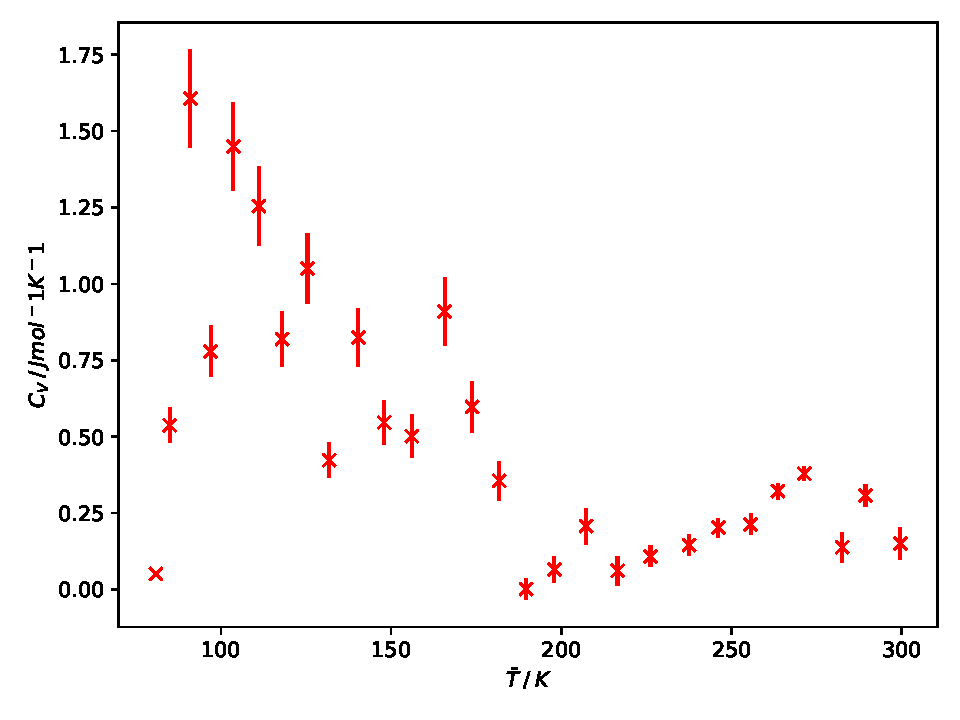
\includegraphics{content/plot1.pdf}
  \caption{Molwärme $C_V$ aufgetragen gegen die durchschnittliche Temperatur $\bar{T}$ im jeweiligen Intervall.}
  \label{fig:plot}
\end{figure}

\subsection{Experimentelle Bestimmung der Debye-Temperatur}

Um die Debye-Temperatur $\theta_\text{D}$ zu bestimmen, werden die $\bar{T}$ mit den entsprechenden Werten $\frac{\theta_\text{D}}{T}$ \cite{Anleitung} multipliziert. 
Die Ergebnisse sind in Tabelle \ref{tab:mess3} zu sehen.\\

\begin{table}
    \centering
    \caption{Experimentell bestimmte Werte für die Debye-Temperatur $\theta_\text{D}$.}
    \label{tab:mess3}
    \sisetup{table-format=2.1}
    \begin{tabular}{c c c}
    \toprule
    $\bar{T} \,/\, \si{\kelvin}$ & $\frac{\theta_\text{D}}{T}$ & $\theta_\text{D} \,/\, \si{\kelvin}$\\
    \midrule 
         80,94 & 15,8 & 1238,34\\
         84,95 & 10,6 &  900,43\\
         90,97 & 13,6 & 1237,23\\
         97,02 & 11,0 & 1067,18\\
        103,67 & 11,5 & 1192,20\\
        111,18 & 13,3 & 1478,72\\
        118,00 & 12,2 & 1439,63\\
        125,44 & 16,2 & 2032,20\\
        131,83 & 13,3 & 1753,34\\
        140,41 & 15,2 & 2134,19\\
        147,93 & 15,7 & 2322,48\\
        156,08 & 12,9 & 2013,48\\
        165,73 & 14,8 & 2452,86\\
    \bottomrule
    \end{tabular}
\end{table}

Der Mittelwert aller bestimmten Debye-Temperaturen $\theta_\text{D}$ ergibt sich zu 

\begin{equation*}
    \bar{\theta_\text{D}} = \SI{1635+-491}{\kelvin}.
\end{equation*}

\subsection{Theoriewert der Debye-Temperatur}

Die Debye-Temperatur lässt sich mit \eqref{eqn:Natome} und \eqref{eqn:Debye} berechnen. Hierzu werden die Werte $v_\text{long} = \SI{4.7}{\kilo\meter\per\second}$ und
$v_\text{trans} = \SI{2.26}{\kilo\meter\per\second}$ \cite{Anleitung} verwendet. Daraus ergibt sich die Schallgeschwindigkeit zu 

\begin{align*}
    \frac{1}{v_\text{s}^3} &= \frac{1}{3} \sum_{i=1}^3 \frac{1}{v_1^3}\\
    \rightarrow v_\text{s} &= \SI{2.54}{\kilo\meter\per\second}. 
\end{align*}

Das Volumen $L^3$ berechnet sich mit 

\begin{equation*}
    L^3 = \frac{m}{\rho}
\end{equation*}

und die Teilchenzahl $N$ mit 

\begin{equation*}
    N = \frac{m}{M}\cdot N_\text{A},
\end{equation*}

wodurch sich $w_\text{D} = \SI{43.5}{\tera\hertz}$ und schließlich 

\begin{equation*}
    \theta_\text{D,theo.} = \SI{332.6}{\kelvin}
\end{equation*}

ergibt.